%\documentclass[notes]{beamer}	   % print frame + notes
%\documentclass[notes=only]{beamer}   % only notes
\documentclass{beamer}			  % only frames

\usetheme{Dresden}
\usecolortheme{orchid}
\usepackage{natbib}
\usepackage[export]{adjustbox}


% These are the configurable settings
% Please change them to make it fit your course
\def \institute {Institute / project name}
\def \authors { Youri Hoogstrate, \institute }

\def \servers {
\begin{itemize}
	\item \url{https://usegalaxy.org/}
	\item \url{https://bioinf-galaxian.erasmusmc.nl/galaxy/}
\end{itemize}
}
\def \datalibrarydirintroduction {
	TraIT Galaxy Training Materials
		$\rightarrow$
	TraIT Galaxy Training - 1: Introduction to Galaxy
}

\def \datalibrarydirrnaseqtuxedo {
	TraIT Galaxy Training Materials
		$\rightarrow$
	TraIT Galaxy Training - 3: RNASeq Tuxedo Pipeline
}

\def \datalibrarydirrnaseqadvanced {
	TraIT Galaxy Training Materials
		$\rightarrow$
	TraIT Galaxy Training - 5: Advanced RNA-Seq Analysis
}
% Configurations should be changed in this file


\title[RNA-Seq (advanced)]{RNA-Seq (advanced)}
\subtitle{Advanced and alternative tools}
%\author[\authors]
%\institute[\institutes]
\subject{Bioinformatics}


\setbeamercolor{footlinecolor}{fg=white,bg=UniBlue}
\makeatletter
\setbeamertemplate{footline}
{
\leavevmode%
\hbox{%
	\begin{beamercolorbox}[wd=.2\paperwidth,ht=0.6cm,left]{bg=white}
%			\includegraphics[scale=0.3]{erasmusLogo.png}
  	\end{beamercolorbox}%
  	\begin{beamercolorbox}[wd=.6\paperwidth,ht=2.25ex,dp=1ex,center]{section in head/foot}%
			\usebeamerfont{title,data}RNA-Seq analysis in Galaxy{ }{ }{ }\insertshortdate
  \end{beamercolorbox}%
  \begin{beamercolorbox}[wd=.2\paperwidth,ht=0.9cm,dp=1ex,center]{bg=white}%
%	\includegraphics[scale=0.27]{trait.png}
  \end{beamercolorbox}}%
  \vskip0pt%
}
\makeatother

\begin{document}
\begin{frame}
	\titlepage % Print the title page as the first slide
\end{frame}

\begin{frame}
	\frametitle{Overview} % Table of contents slide, comment this block out to remove it
	\begin{scriptsize}
		\tableofcontents
	\end{scriptsize}
\end{frame}

\section{Introduction} % Biology + Methodology
\subsection{RNA-Seq}
\begin{frame}
	\frametitle{Central dogma}
	\begin{center}
		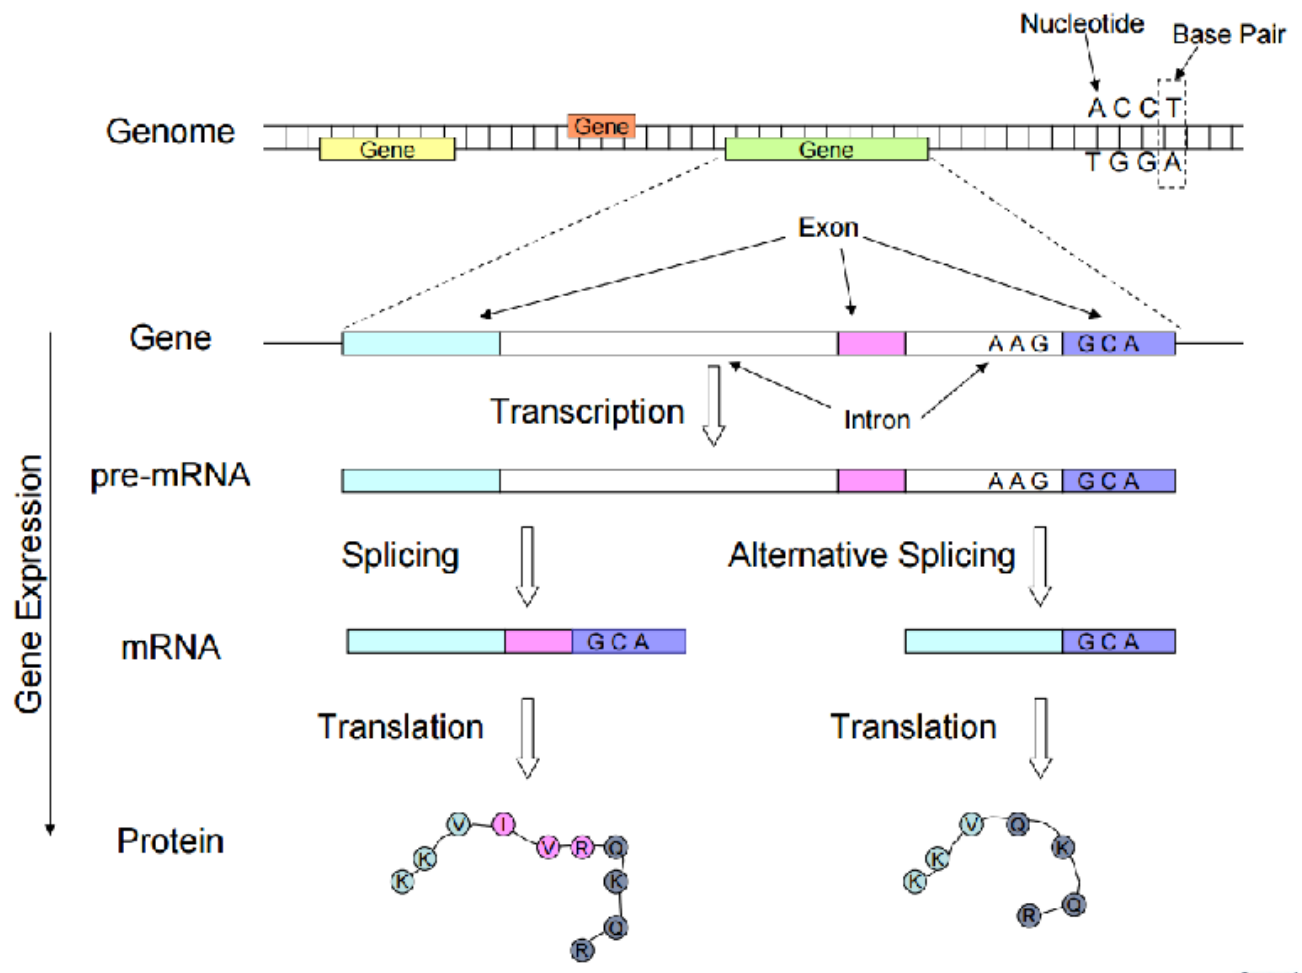
\includegraphics[height=0.8\textheight]{figures/dge_00ap.png}
	\end{center}
\end{frame}

\begin{frame}
	\frametitle{Central dogma}
	\begin{center}
		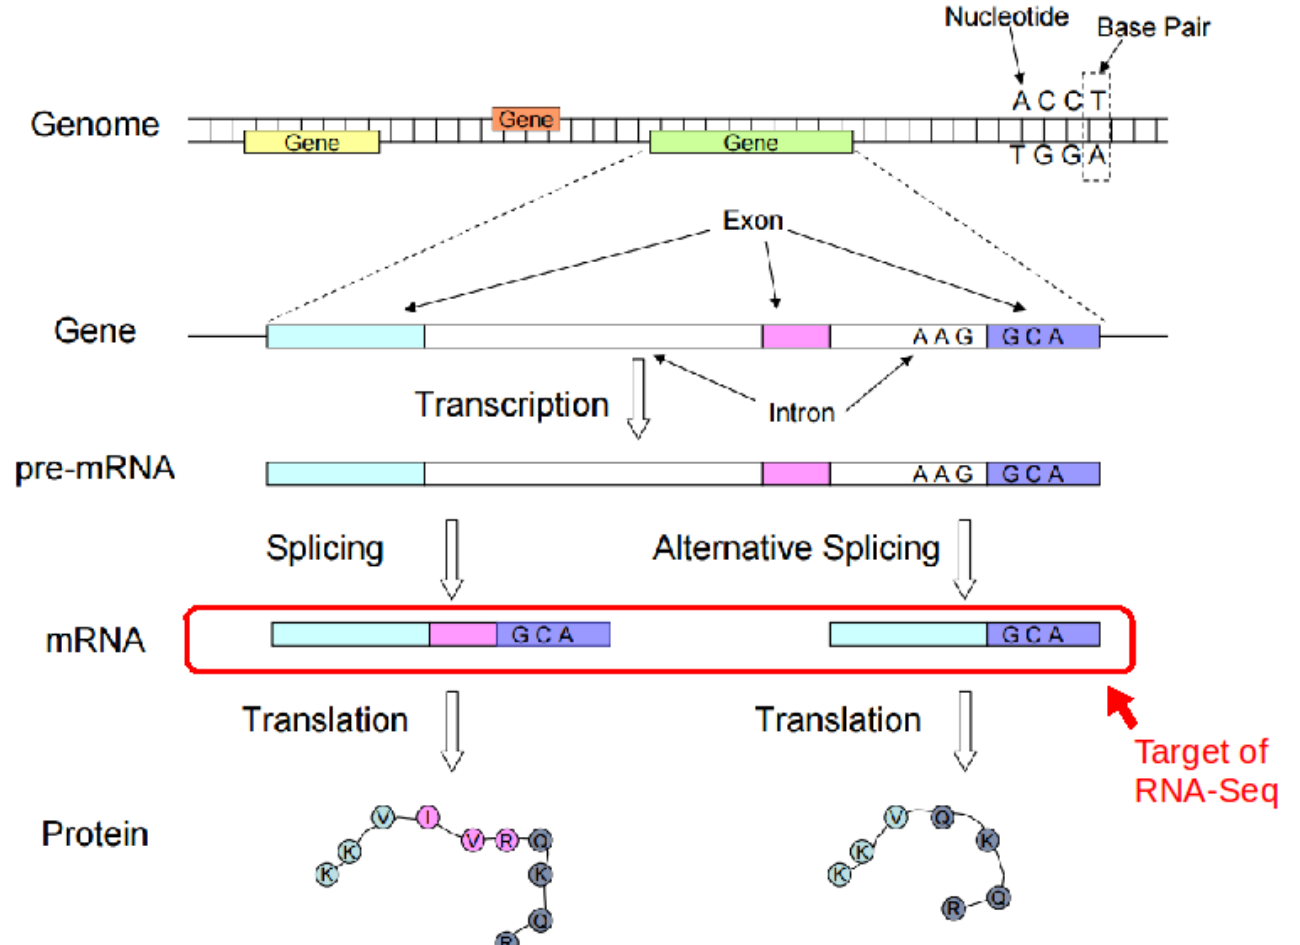
\includegraphics[height=0.8\textheight]{figures/dge_00bp.png}
	\end{center}
\end{frame}

\begin{frame}
	\frametitle{RNA-Seq}
	\begin{center}
		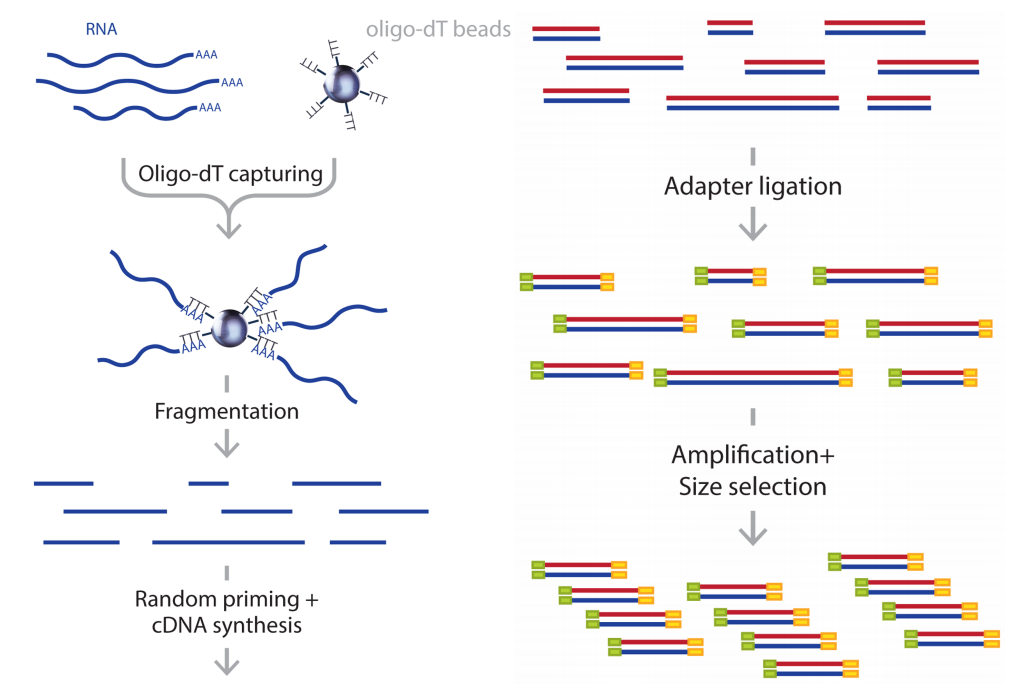
\includegraphics[height=0.8\textheight]{figures/dge_01ap.png}
	\end{center}
\end{frame}

\begin{frame}
	\frametitle{RNA-Seq}
	\begin{center}
		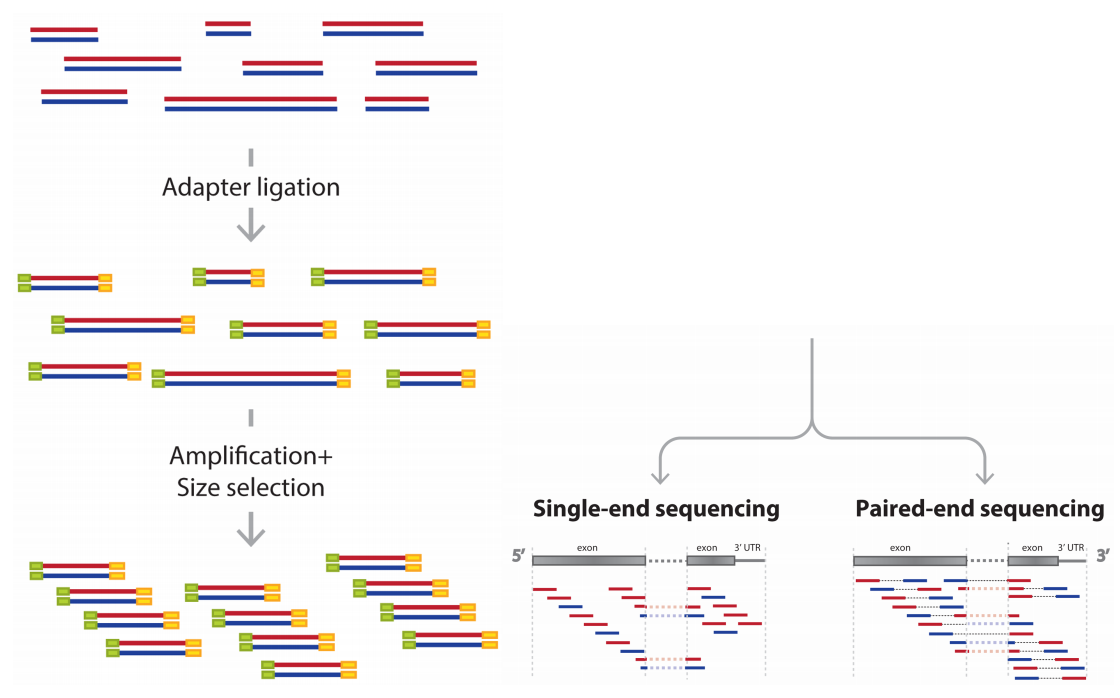
\includegraphics[height=0.8\textheight]{figures/dge_01bp.png}
	\end{center}
\end{frame}

\begin{frame}
\frametitle{Sequencer: HiSeq}
  \begin{columns}[T]
	\begin{column}{.62\textwidth}
	\begin{itemize}
		\item High throughput
		\item Paired end
		\item High accuracy
		\item Read length 2$\times$150bp
		\item Relatively long run time
		\item Relatively expensive
	\end{itemize}
	\end{column}
	\begin{column}{.38\textwidth}
		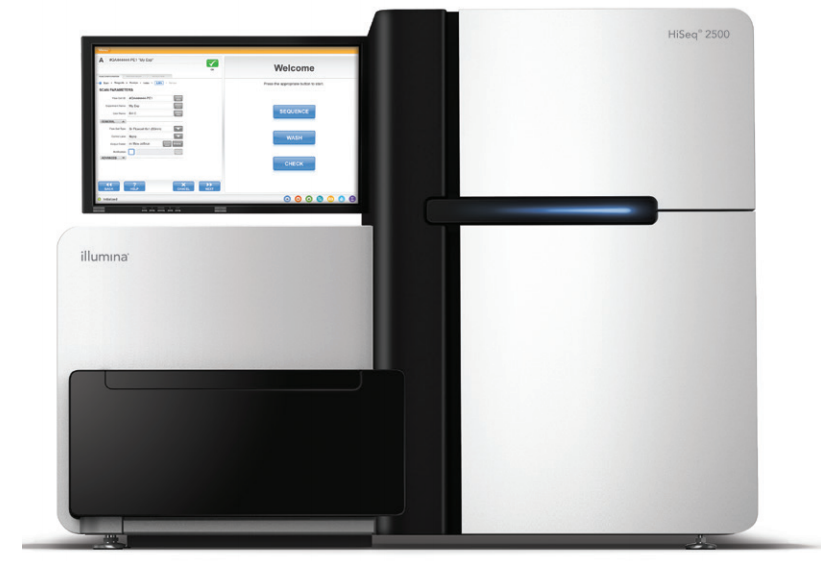
\includegraphics[width=\textwidth]{figures/dge_02p.png}
	\end{column}
  \end{columns}
\end{frame}

\begin{frame}
	\frametitle{FASTQ file format}
	\begin{itemize}
		\item Sequence is given per char
		\begin{itemize}
			\item Two corresponding files (often ``R1”, ``R2”)
			\item[ ] \quad
		\end{itemize}
	\end{itemize}
	\begin{center}
		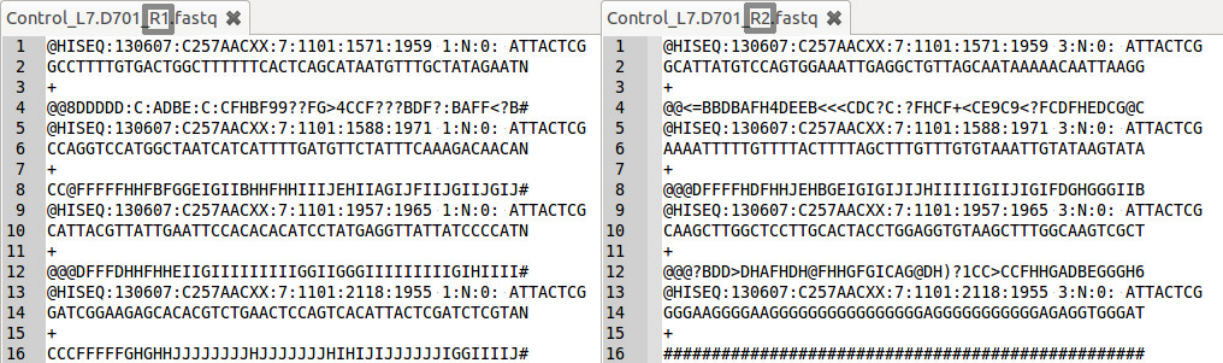
\includegraphics[width=\textwidth]{figures/dge_03ap.png}
	\end{center}
\end{frame}

\begin{frame}
	\frametitle{FASTQ file format}
	\begin{itemize}
		\item Sequence is given per char
		\begin{itemize}
			\item Two corresponding files (often ``R1”, ``R2”)
			\item Pairs linked by position in file (and name)
		\end{itemize}
	\end{itemize}
	\begin{center}
		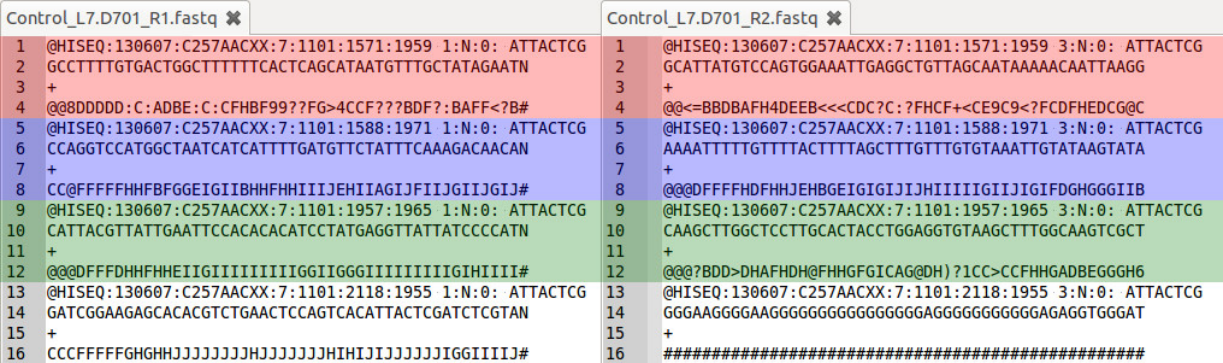
\includegraphics[width=\textwidth]{figures/dge_03bp.png}
	\end{center}
\end{frame}

\begin{frame}
	\frametitle{FASTQ file format}
	\begin{itemize}
		\item Sequence is given per char
		\begin{itemize}
			\item N means \textit{sequencer doesn’t know}
		\end{itemize}
		\item Quality is encoded as a char
		\begin{itemize}
			\item reflects probability of being called correctly
		\end{itemize}
		\item Different encodings
		\begin{itemize}
			\item {\scriptsize \url{https://en.wikipedia.org/wiki/FASTQ\_format\#Encoding}}
		\end{itemize}
	\end{itemize}
	\begin{center}
		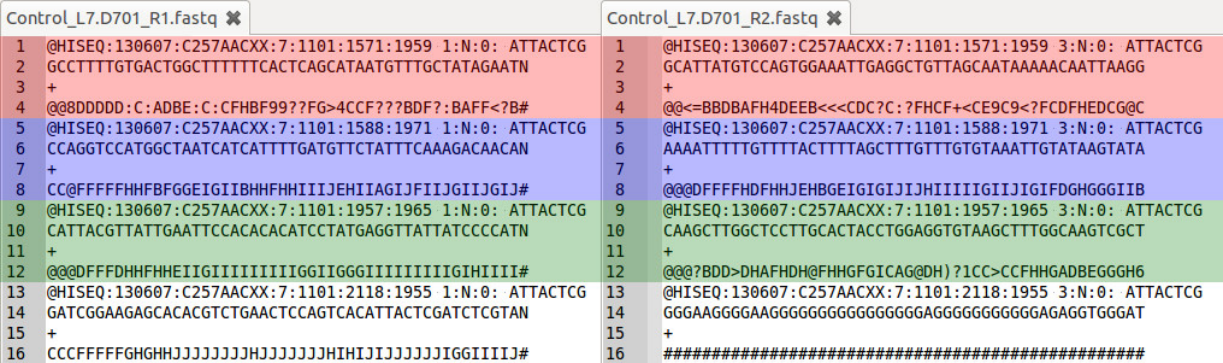
\includegraphics[width=\textwidth]{figures/dge_03bp.png}
	\end{center}
\end{frame}

\begin{frame}
\frametitle{General RNA-seq expression profiling pipeline}
  \begin{columns}[T]
	\begin{column}{.72\textwidth}
	\begin{itemize}
		\item Pre-alignment
		\begin{itemize}
			\item QC
			\item Data cleaning
		\end{itemize}
		\item Alignment
		\begin{itemize}
			\item Use special RNA-Seq aligner
		\end{itemize}
		\item Transcript assembly
		\begin{itemize}
			\item Known transcripts
		\end{itemize}
		\item Expression quantification
		\begin{itemize}
			\item From alignment?
		\end{itemize}
		\item Hypothesis testing
	\end{itemize}
	\end{column}
	\begin{column}{.28\textwidth}
	\end{column}
  \end{columns}
\end{frame}

\note{Differentially expressed genes may serve as prognostic markers in many diseases. The RNA levels of up- or down-regulated genes. However, they are not the driver events. In cancer, cells keep on evolving and those mutations that have positive effects on genes that relate to cell replication. Therefore the expression levels can serve as indicator. Because we have near 22.000 protein coding genes, and many genes directly interact with other genes, a cell has many alternative interaction routes to accomplish and control messages. Therefore, differential expression is often not a matter of one gene but of a series of genes that have interaction with each other. } 

\begin{frame}
\frametitle{Quality assurance \& quality control}
  \begin{columns}[T]
	\begin{column}{.72\textwidth}
	\begin{itemize}
		\item FastQC
		\begin{itemize}
			\item GC content and distribution
			\item Quality score distribution
			\item Adapter sequence contamination
		\end{itemize}
		\item Trimmomatic and Sickle
		\begin{itemize}
			\item Remove linker/adapter sequences
			\item Trim low quality reads at the ends
			\item Evaluate the part of the read that remains
		\end{itemize}
	\end{itemize}
	\end{column}
	\begin{column}{.28\textwidth}
	\end{column}
  \end{columns}
\end{frame}

\begin{frame}
\frametitle{FastQC}
\framesubtitle{Base quality report}
	\begin{center}
		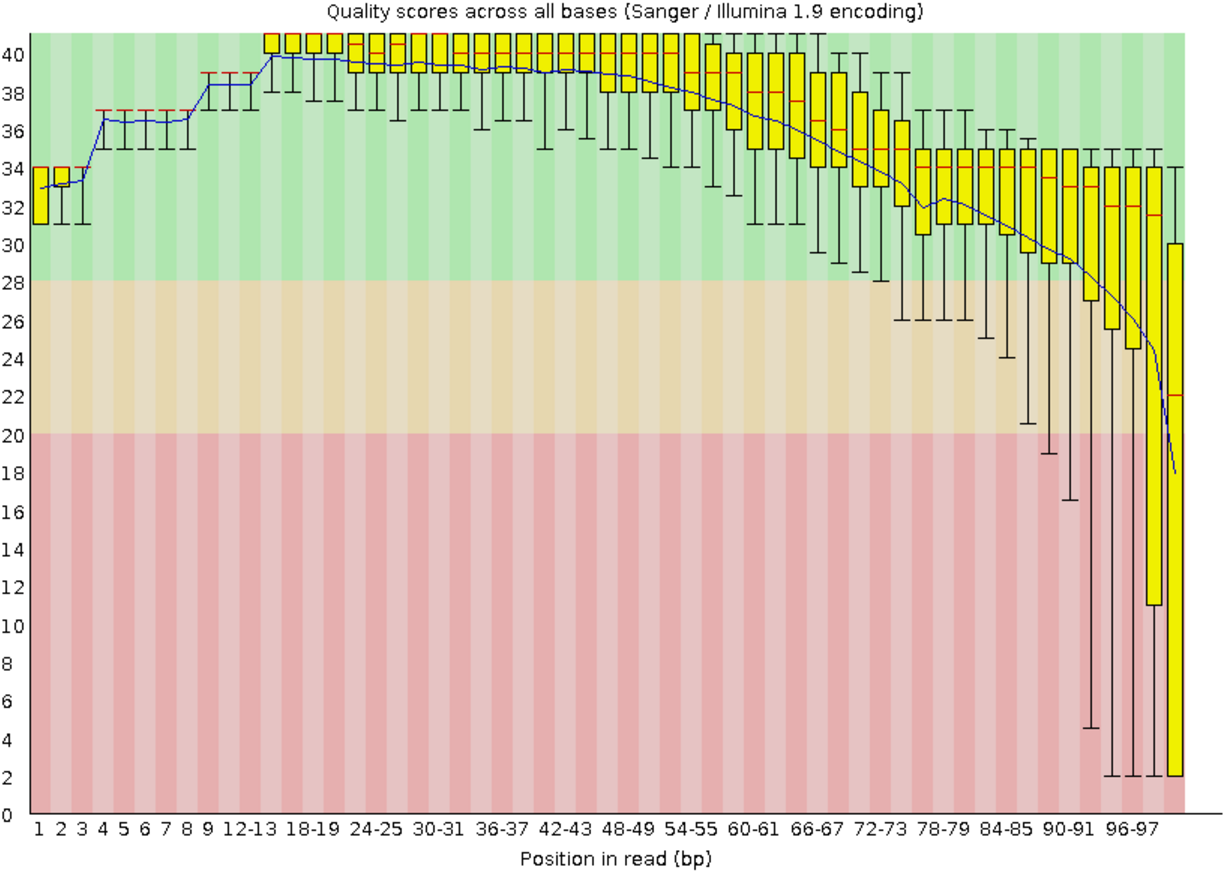
\includegraphics[height=0.75\textheight]{figures/dge_03cp.png}
	\end{center}
\end{frame}

\begin{frame}
\frametitle{Quality assurance \& quality control}
	\begin{itemize}
		\item Trim low quality bases from the ends
		\begin{itemize}
			\item Paired end data: reads are linked by position in
files
			\item Proceed with trimmed reads
		\end{itemize}
	\end{itemize}
	\begin{center}
		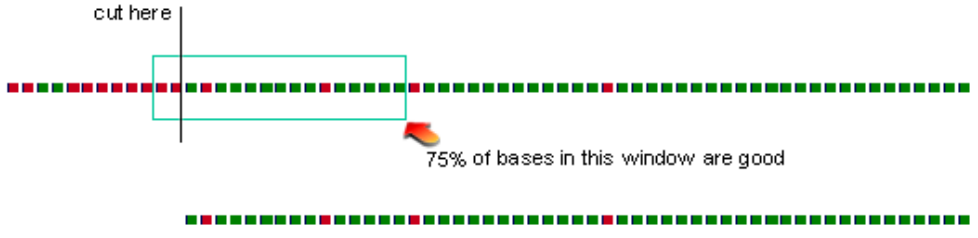
\includegraphics[width=\textwidth]{figures/dge_03dp.png}
	\end{center}
\end{frame}


\begin{frame}
\frametitle{FastQC}
\framesubtitle{Base adapter contamination}
	\begin{center}
		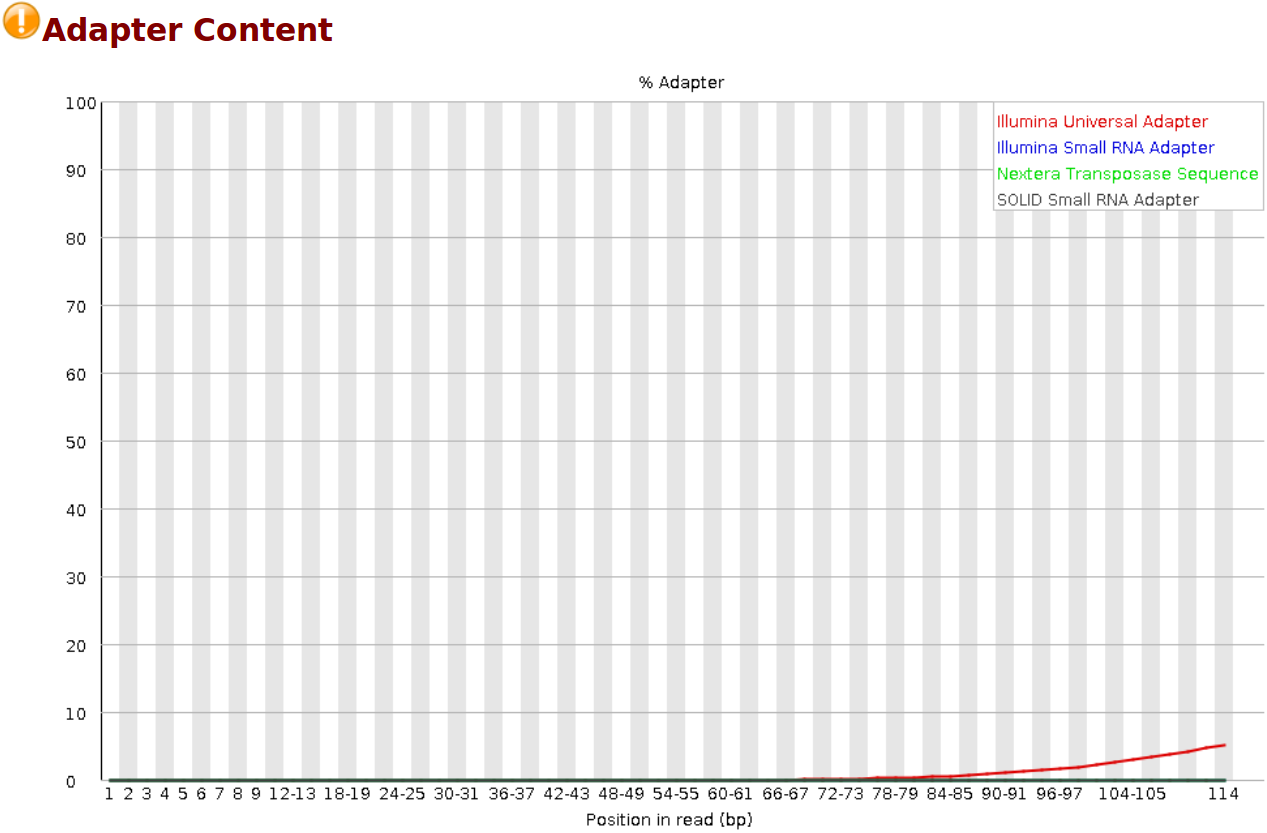
\includegraphics[height=0.75\textheight]{figures/dge_04p.png}
	\end{center}
\end{frame}

\begin{frame}
\frametitle{Alignment}
\framesubtitle{Exons, introns, gap penalties}
	\begin{center}
		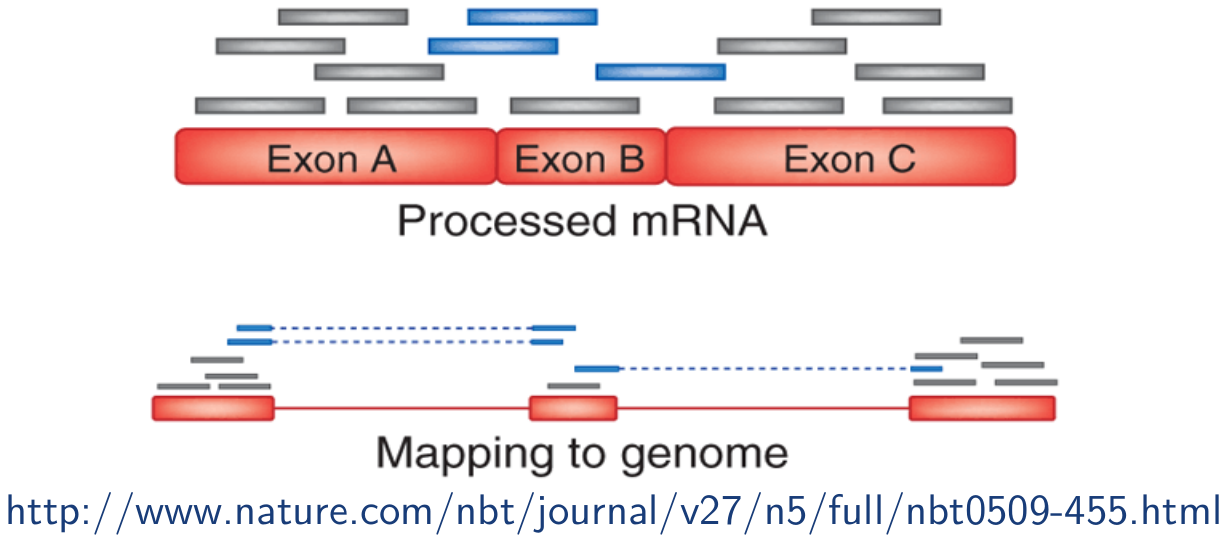
\includegraphics[width=\textwidth]{figures/dge_05p.png}
	\end{center}
\end{frame}

\begin{frame}
\frametitle{Alignment tools}
\framesubtitle{Exons, introns, gap penalties}
	\begin{center}
		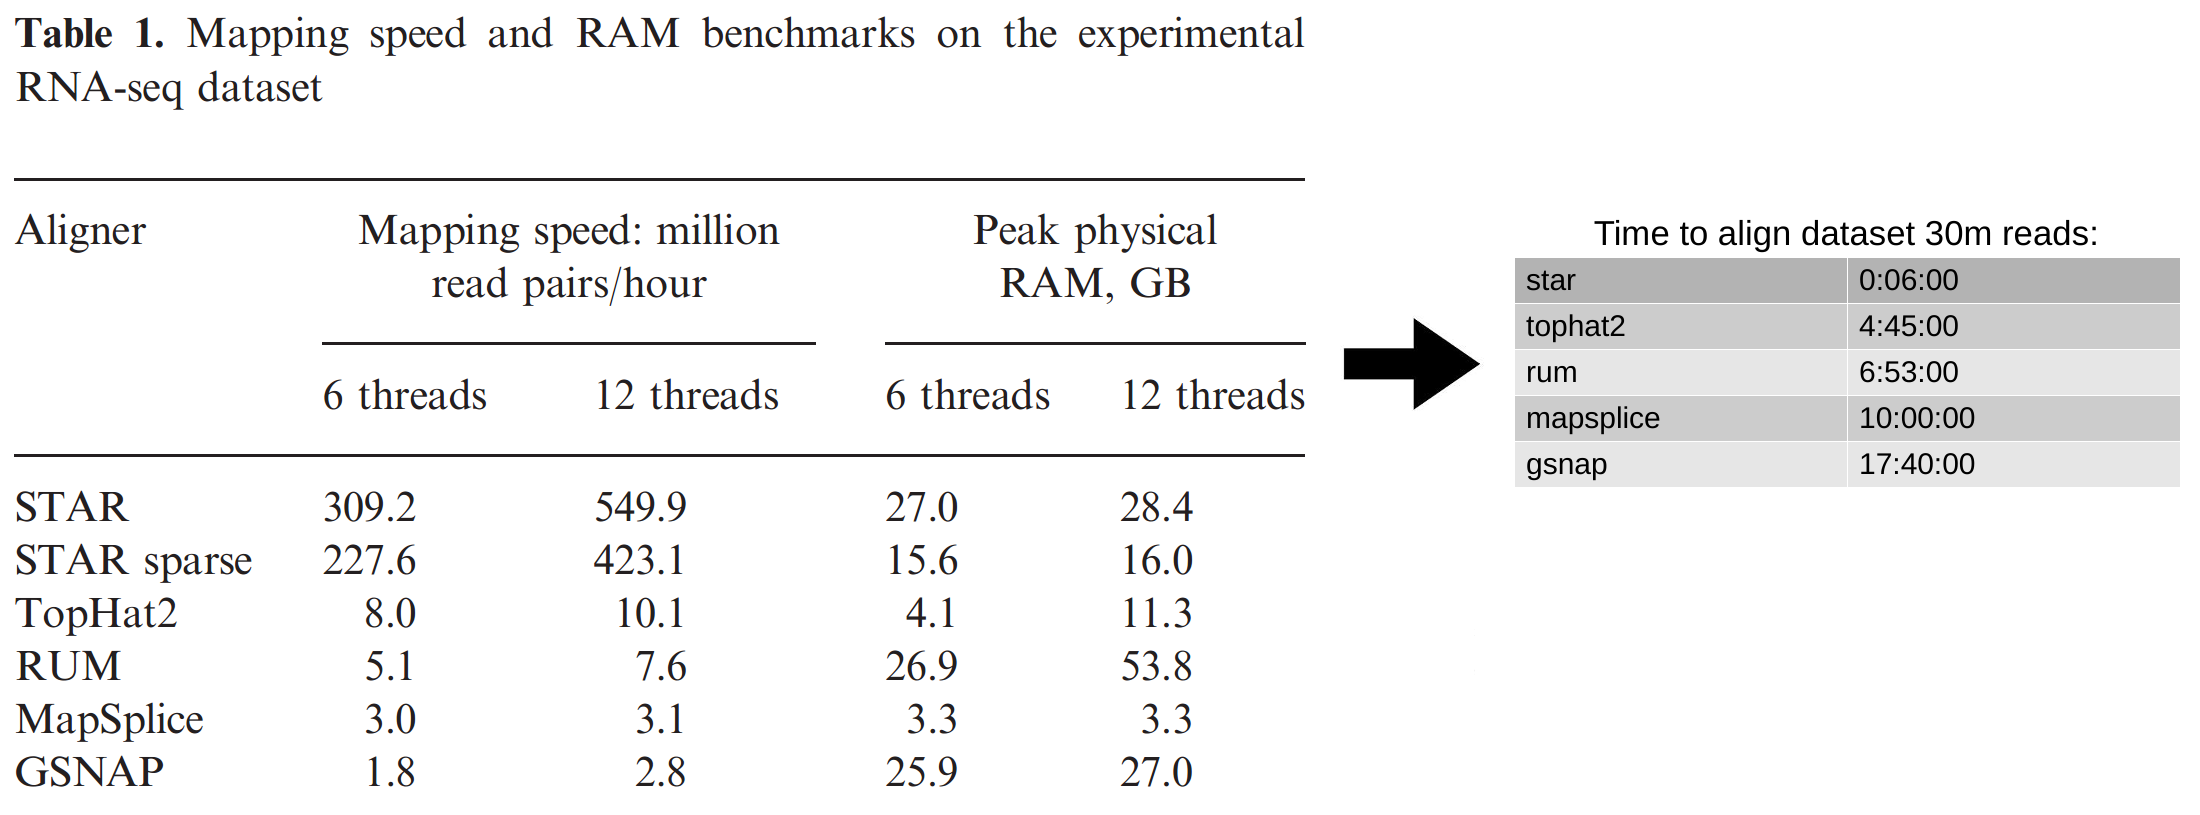
\includegraphics[width=\textwidth]{figures/dge_06p.png}\\\cite{star}
	\end{center}
\end{frame}


\begin{frame}
\frametitle{Alignment tools}
\framesubtitle{Currently most used}
	\begin{itemize}
		\item RNA-STAR\cite{star}
		\item HISAT2\cite{hisat}
	\end{itemize}
\end{frame}

\section{Tuxedo pipeline}

\begin{frame}
	\frametitle{Differential gene expression}
	\framesubtitle{}
	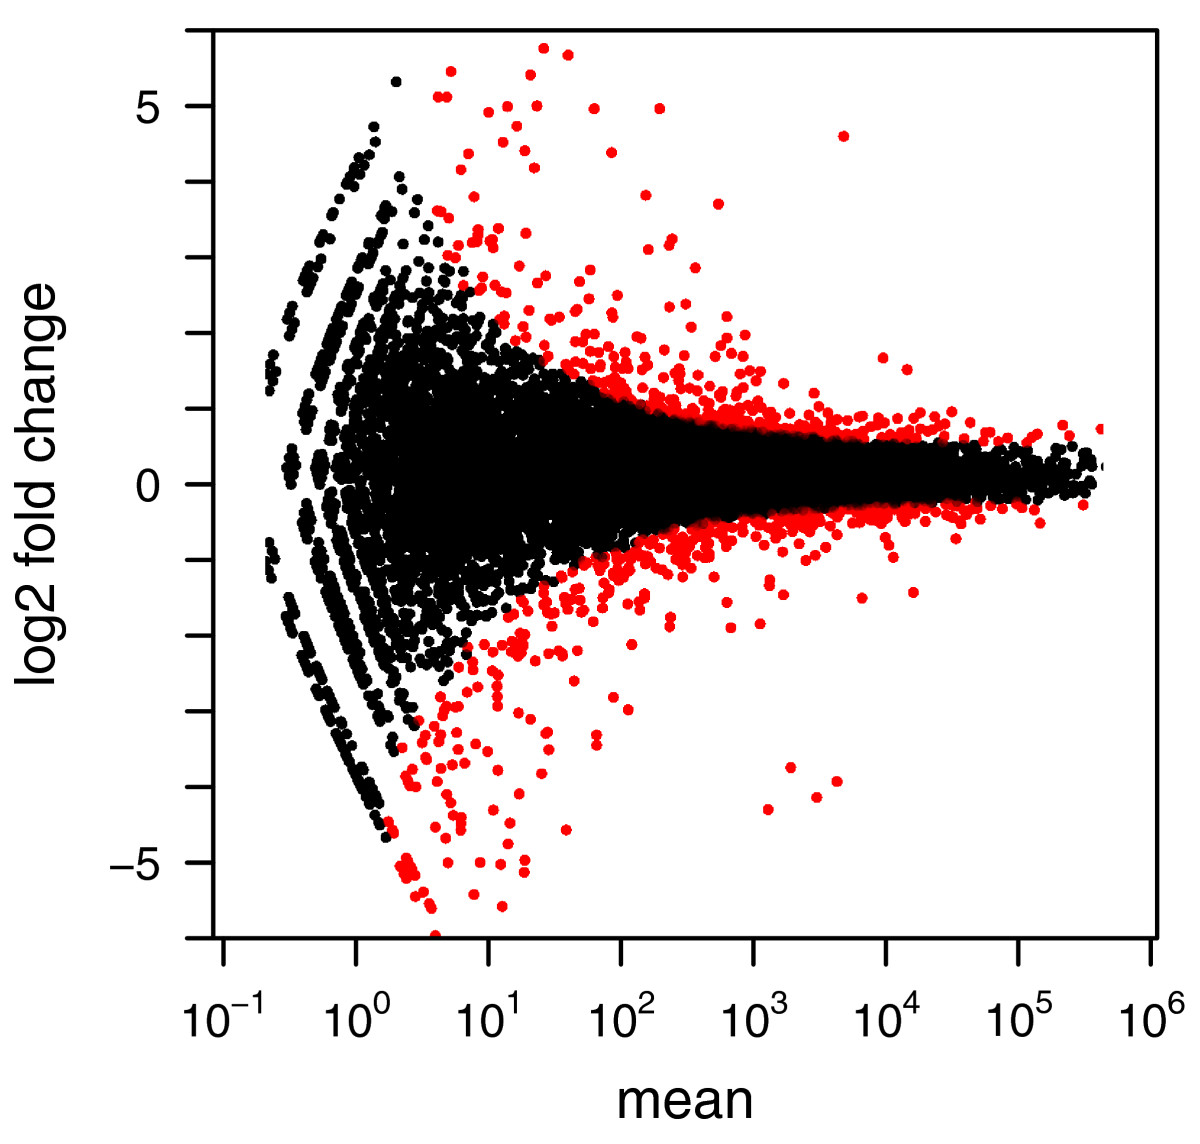
\includegraphics[width=0.35\textwidth]{figures/diff_expr.jpg}\\
	\begin{itemize}
		\item Triggered by
		\begin{itemize}
			\item Stimuli (signal molecules)
			\item Genetics (mutation)
		\end{itemize}
		\item Genes interact in a network, effect spreads out
		\begin{itemize}
			\item Genetic redundancy / biological robustness (often multiple changes necessary to cause a disease)
		\end{itemize}
	\end{itemize}
\end{frame}
  
\begin{frame}
\frametitle{Tuxedo pipeline}
\framesubtitle{TopHat, Cufflinks, CuffMerge, CuffDiff, CummeRbund}
	\begin{center}
		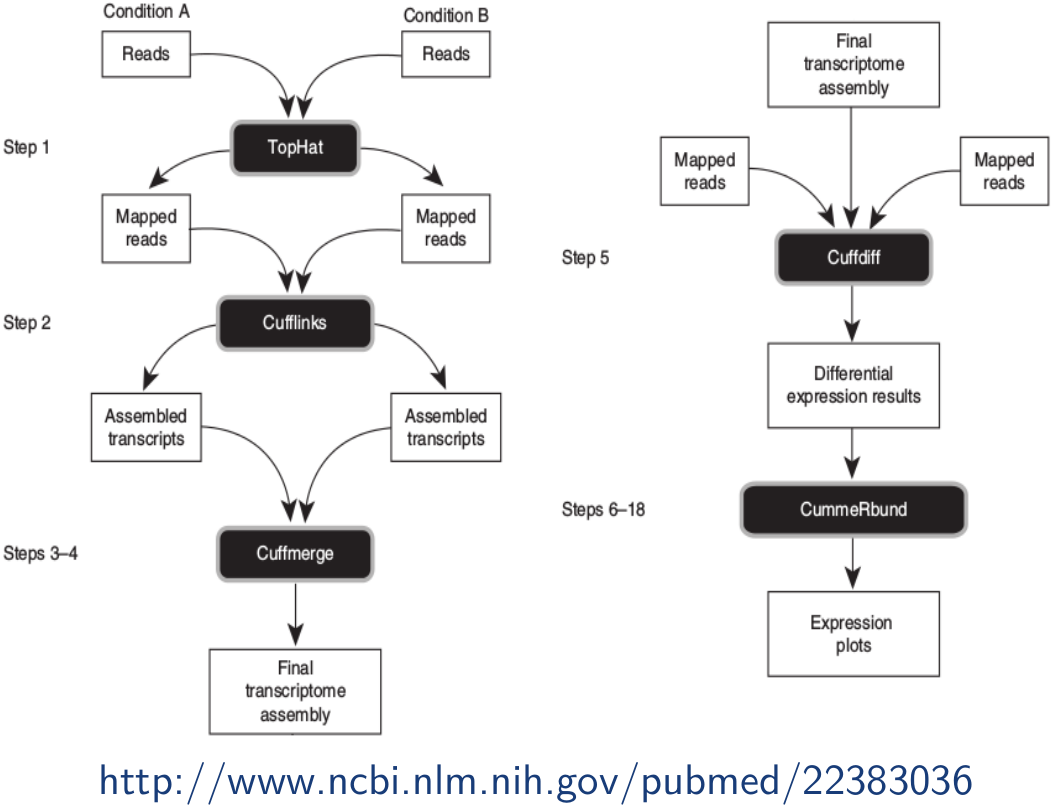
\includegraphics[height=0.75\textheight]{figures/dge_07p.png}
	\end{center}
\end{frame}

\begin{frame}
\frametitle{Tuxedo pipeline}
\framesubtitle{TopHat, Cufflinks, CuffMerge, CuffDiff, CummeRbund}
	\begin{itemize}
		\item CuffLinks
		\begin{itemize}
			\item Estimate transcript abundance
			\item Assemble transcripts (incl. novel)
		\end{itemize}
		\item CuffMerge
		\begin{itemize}
			\item Merge novel and known gene annotations
		\end{itemize}
		\item CuffDiff
		\begin{itemize}
			\item Test hypothesis, find diff. expressed genes/transcripts
		\end{itemize}
		\item CummeRbund
		\begin{itemize}
			\item Static visualizations
		\end{itemize}
	\end{itemize}
\end{frame}


\section{Advanced (DGE) analysis}

\begin{frame}
\frametitle{Tuxedo pipeline}
\framesubtitle{Limitations}
	\begin{itemize}
		\item ``Paired'' designs: tumor and normal from same patient, batch effects
		\item Less control (e.g. use additional class-label for normalization but exclude it from the test)
	\end{itemize}
\end{frame}

\begin{frame}
\frametitle{Generic RNA-Seq workflow}
	\begin{center}
		%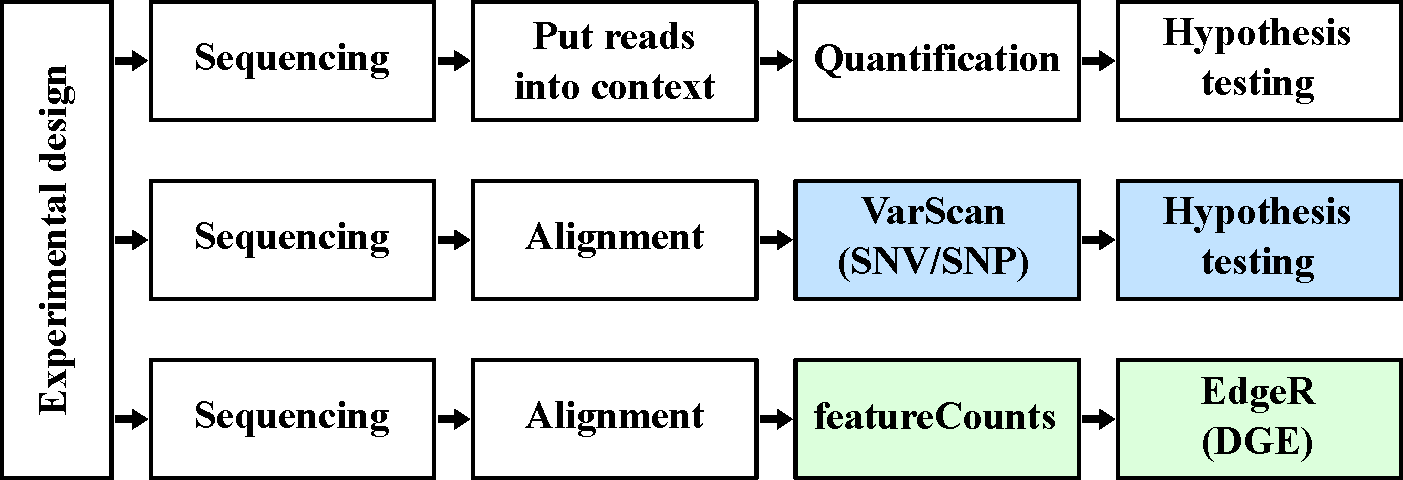
\includegraphics[width=\textwidth]{figures/dge_08p.pdf}
	\end{center}
\end{frame}

\note{Virtually all types of analysis follow the above workflow, assuming we have high quality data at our starting point. There are some exceptions, but those usually merge two blocks into one block.}

\subsection{Quantification}
\begin{frame}
	\frametitle{Measure expression levels in RNA-Seq data}
	\begin{itemize}
			\item Align read to reference genome
		\item Measuring expression = counting aligned reads
		\begin{itemize}
				\item Count in annotated exons
			\item Positive integers (read count of 3.1415 or $-42 = $ \textbf{impossible})
			\item Quantitative (read count has an absolute meaning)
		\end{itemize}
		\item Observation (read count) must be \textbf{statistically independent}
		\begin{itemize}
			\item No multi-map reads
			\item Skip overlapping gene annotations
		\end{itemize}
	\end{itemize}
	
	\begin{figure}
		%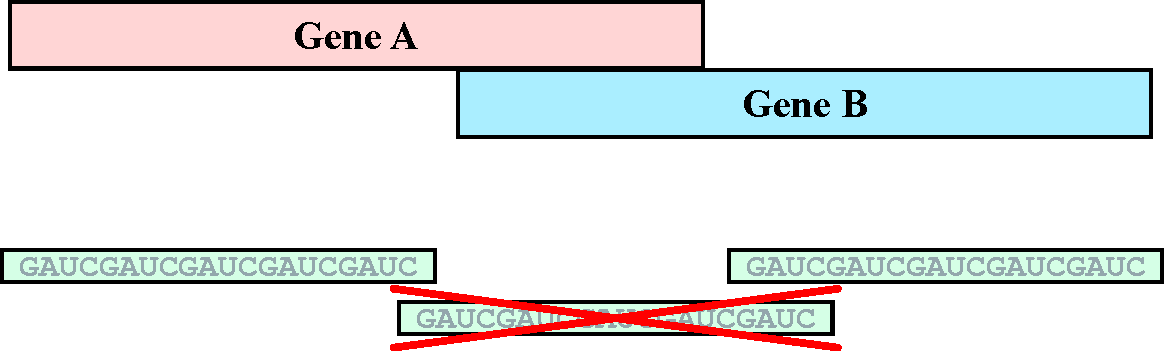
\includegraphics[width=0.5\textwidth]{figures/dge_09p.pdf}
	\end{figure}
	\begin{itemize}
		\item Tools: featureCounts, HTSeq-count \cite{featurecounts,htseq}
	\end{itemize}
\end{frame}


\subsection{Hypothesis testing}

\begin{frame}
	\frametitle{Differential gene expression analysis}
	\framesubtitle{edgeR and DESeq2}
	\begin{itemize}
			\item edgeR or DESeq2\cite{edger,deseq2}
		\begin{itemize}
			\item Free R Packages
		\item Galaxy wrapper does normalizations for you
		\begin{itemize}
			\item Use raw reads, do NOT use FPKM/RPKM!
		\end{itemize}
	\end{itemize}
		\item ``Limma" for count data
		\begin{itemize}
			\item Not Gaussian (normal) distributed like e.g. micro-array data $-$ but negative binomial 
		\end{itemize}
	\end{itemize}
\end{frame}

\begin{frame}
	\frametitle{Differential gene expression analysis - normalization}
	\framesubtitle{edgeR and DESeq2}
	\begin{itemize}
		\item Tests correct for read depth
		\item Tests correct for (over-)dispersion (biological variation)
		\begin{itemize}
			\item Related to read count per gene - highly expressed genes have lower variation
			\begin{itemize}
				\item Related to gene length
			\end{itemize}
		\end{itemize}
	\end{itemize}
\end{frame}

\begin{frame}
\frametitle{Differential gene expression analysis}
\framesubtitle{Read counts: negative binomial distributed}
	\begin{figure}
		%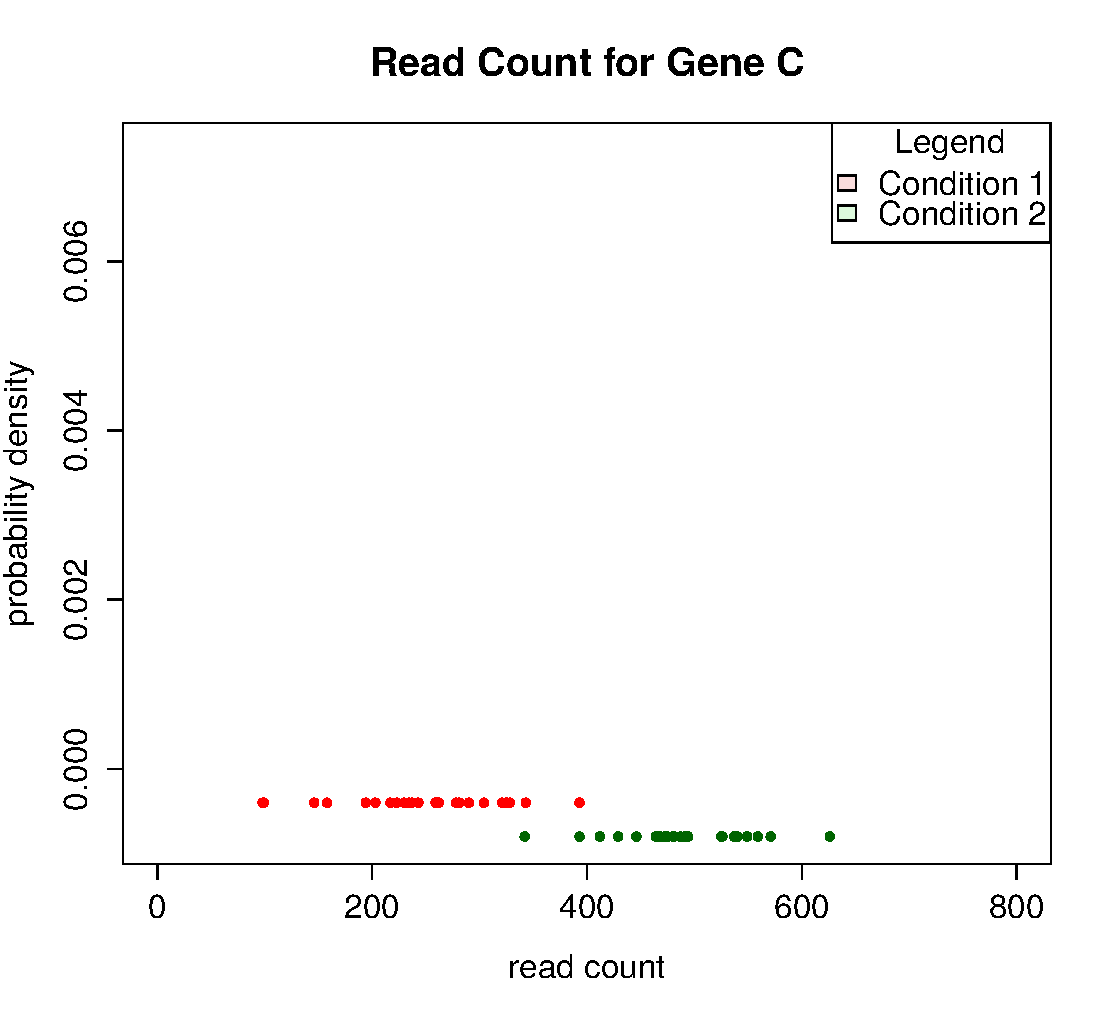
\includegraphics[width=0.60\textwidth]{figures/dge_10ap.pdf}
	\end{figure}
\end{frame}

\begin{frame}
\frametitle{Differential gene expression analysis}
\framesubtitle{Read counts: negative binomial distributed}
	\begin{figure}
		%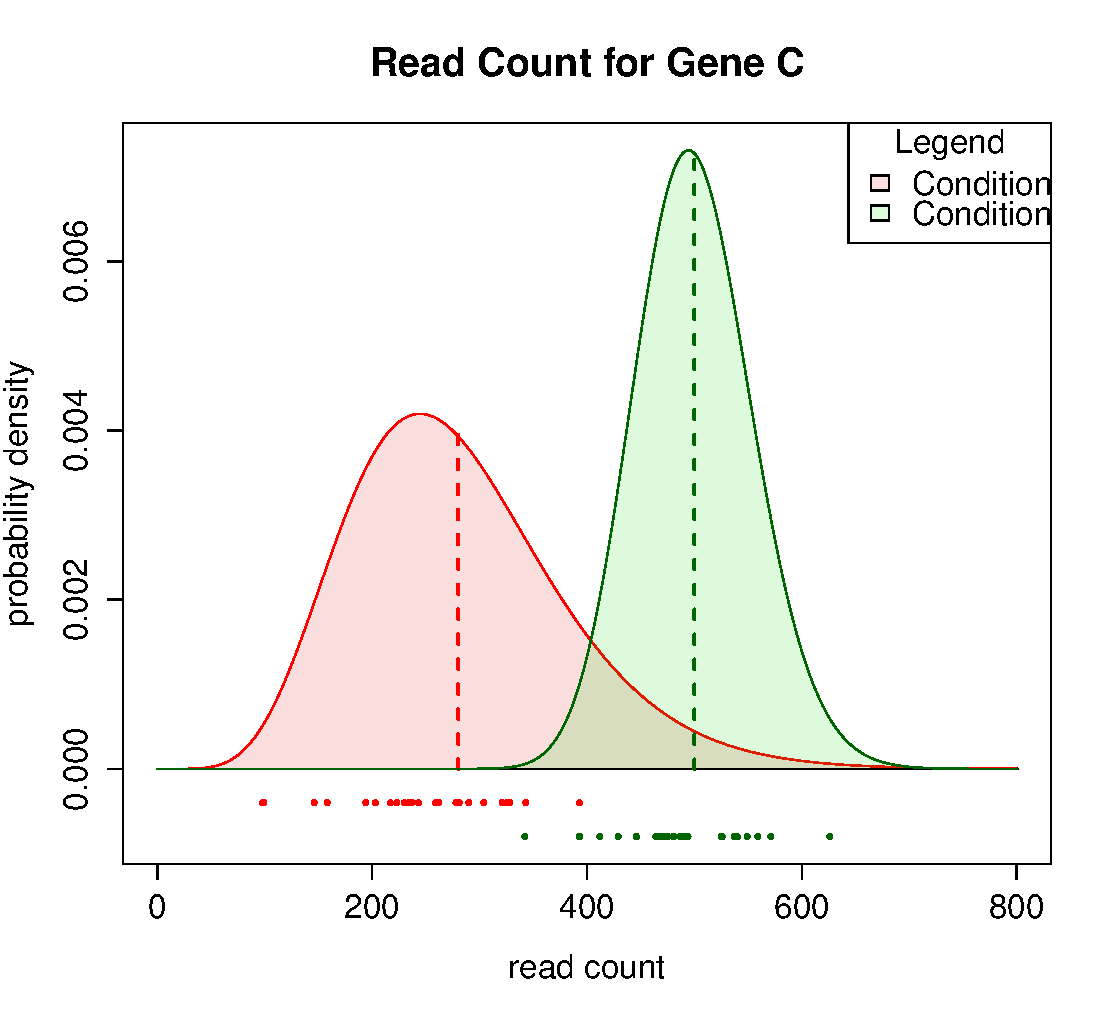
\includegraphics[width=0.60\textwidth]{figures/dge_10bp.pdf}
	\end{figure}
\end{frame}


\begin{frame}
	\frametitle{Differential gene expression analysis}
		%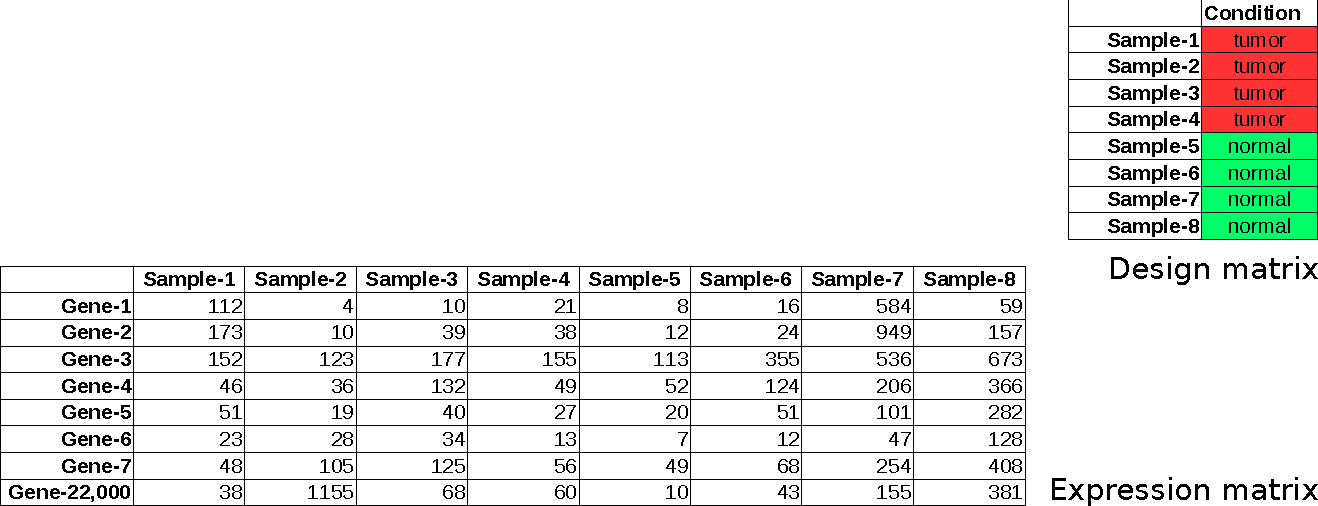
\includegraphics[width=\textwidth]{figures/dge_11ap.pdf} \\
	\textcolor{white}{C}
\end{frame}

\begin{frame}
	\frametitle{Differential gene expression analysis}
		%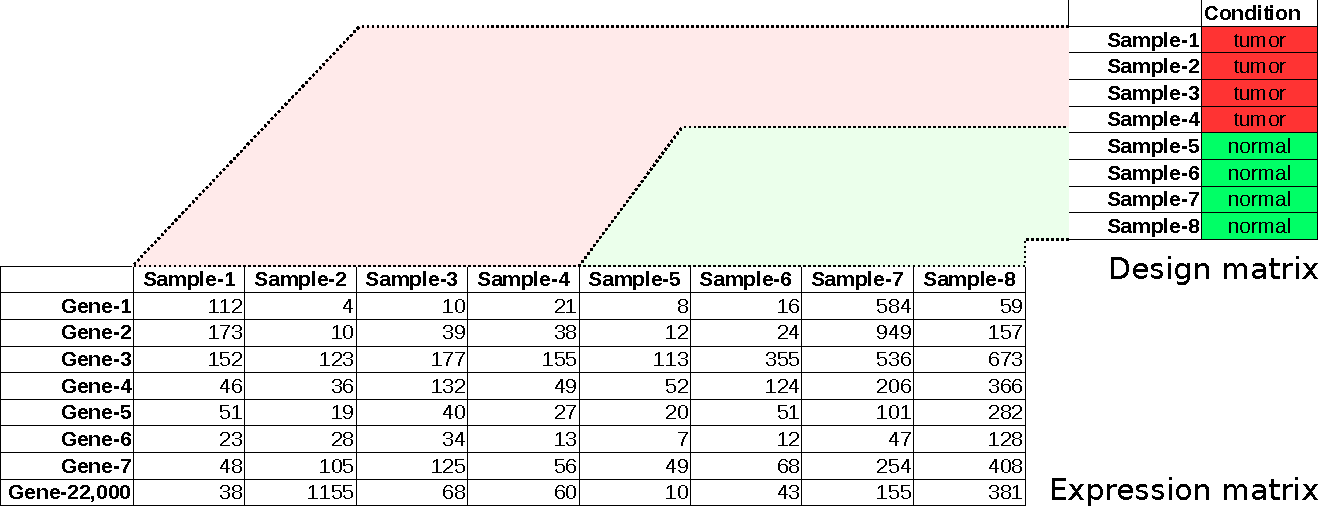
\includegraphics[width=\textwidth]{figures/dge_11bp.pdf} \\
	\textcolor{white}{C}
\end{frame}

\begin{frame}
	\frametitle{Differential gene expression analysis}
		%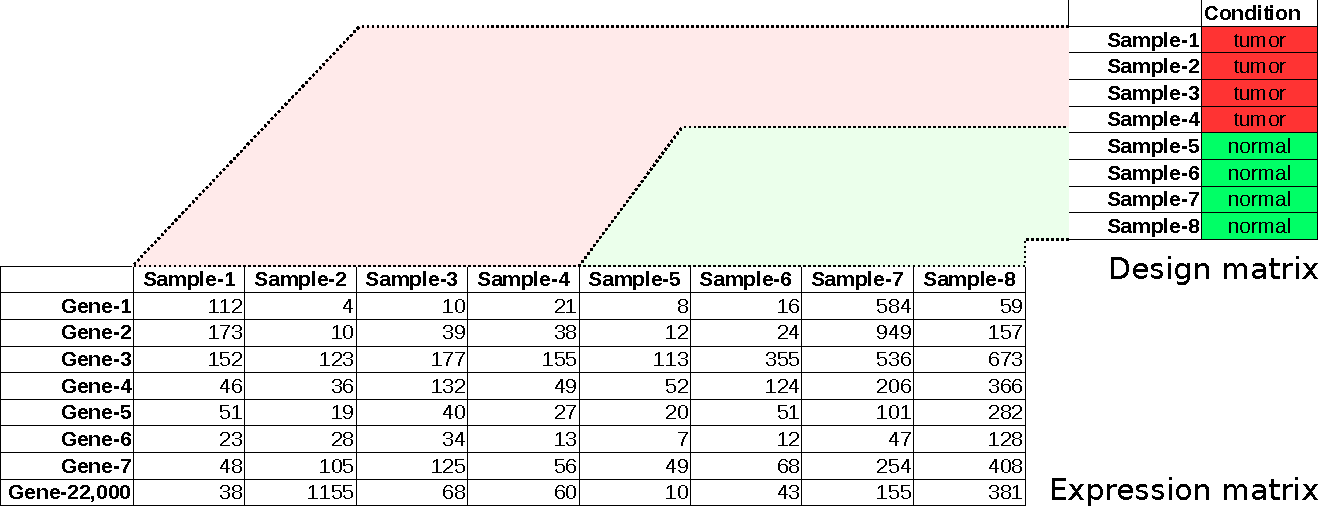
\includegraphics[width=\textwidth]{figures/dge_11bp.pdf} \\
	Contrast = tumor $\leftrightarrow$ normal
\end{frame}

\begin{frame}
	\frametitle{Negative binomial: statistical power}
	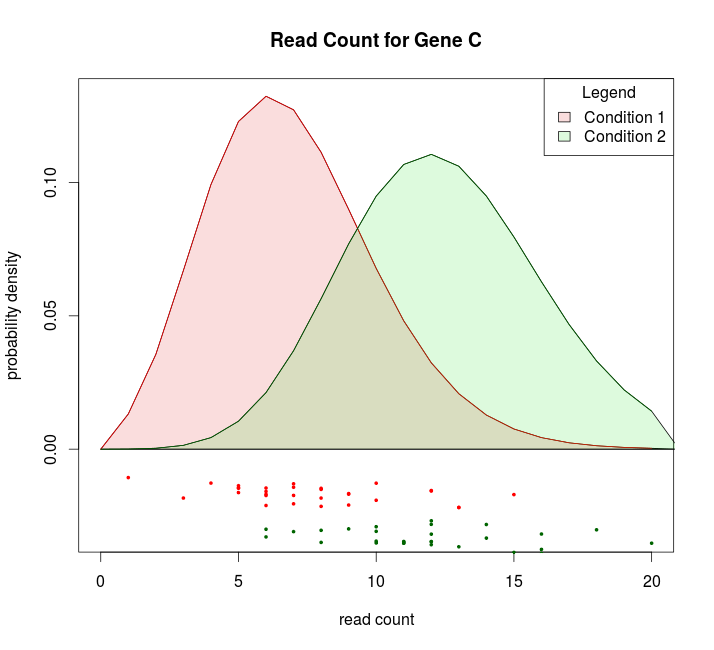
\includegraphics[width=0.33\textwidth]{figures/dge_12ap.png}
	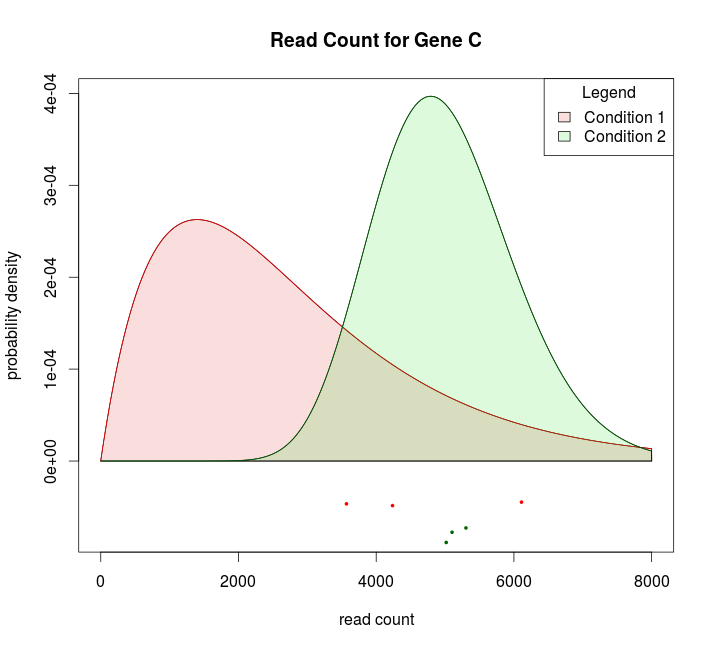
\includegraphics[width=0.33\textwidth]{figures/dge_12bp.png}
	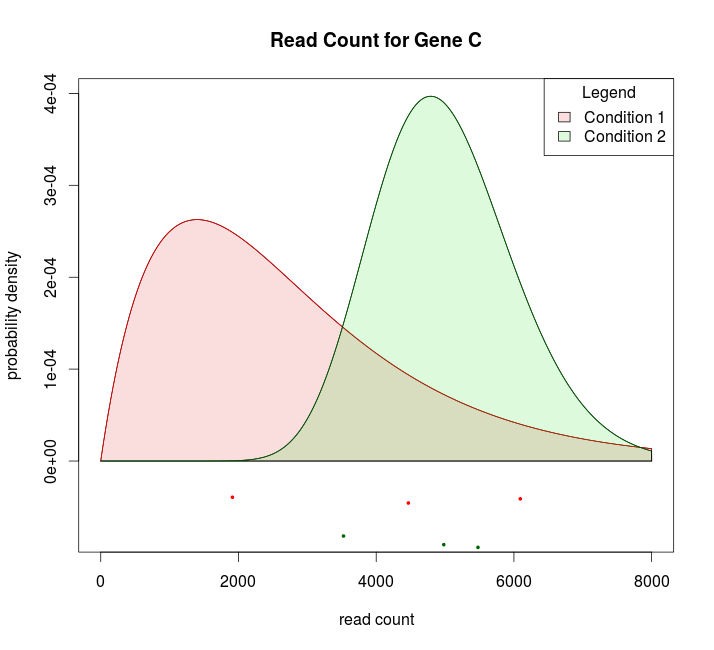
\includegraphics[width=0.33\textwidth]{figures/dge_12cp.png}
	
	\begin{itemize}
		\item Low number of samples complicate estimation of dispersion
		\item Solution (for more power): deeper sequencing, more replicates..?
	\end{itemize}
\end{frame}

\begin{frame}
	\frametitle{Differential gene expression analysis}
	\framesubtitle{Statistical power: MCF7 cell line}
	\begin{itemize}
		\item {\scriptsize\textit{``RNA-seq differential expression studies: more sequence or more replication?''}}\cite{mcf7}:
		\begin{itemize}
			\item MCF7 cell line
			\item 7$\times$treated with E2 hormone, 7$\times$control $\rightarrow$ stimulus known for large response
			\item Each sample sequenced at 30M reads
			\item Study: find number DGE genes
			\begin{itemize}
				\item Vary number of samples: $2-7$
				\item Vary sequencing depth (subset): $5M-30M$
			\end{itemize}			
		\end{itemize}
	\end{itemize}
\end{frame}

\begin{frame}
	\frametitle{Differential gene expression analysis}
	\framesubtitle{Statistical power: MCF7 cell line}
	\begin{center}
		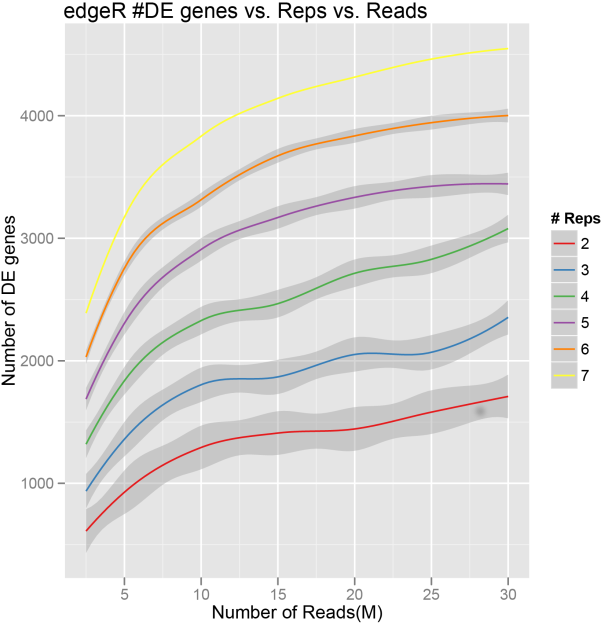
\includegraphics[width=0.45\textwidth]{figures/dge_13ap.png}
		\cite{mcf7}
	\end{center}
\end{frame}

\begin{frame}
	\frametitle{Differential gene expression analysis}
	\framesubtitle{MCF7 cell line}
	\begin{center}
		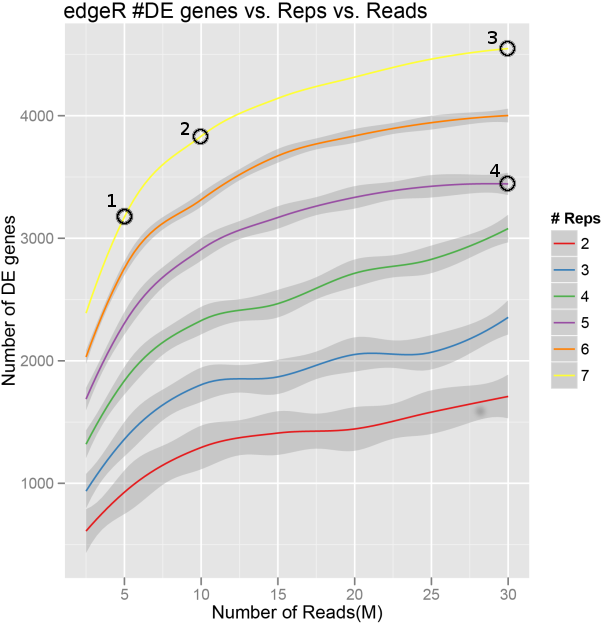
\includegraphics[width=0.45\textwidth]{figures/dge_13bp.png}
		\cite{mcf7}
	\end{center}
\end{frame}

%\subsubsection{Sample pairing}
%\begin{frame}
%	\frametitle{Differential gene expression analysis: sample pairing}
%		\begin{itemize}
%			\item Sample pairing (do not confuse with PE-reads!) / batch effects
%			\item Goal: correction for patient / batch specific expression profiles
%			\item Examples:
%			\begin{itemize}
%				\item $10 \times$Tumour \& Normal (both of same patient)
%				\item 3 populations: African, American \& Asian
%				\item 2 batches: 1 at Monday, 1 at Friday
%			\end{itemize}
%	\end{itemize}
%\end{frame}

%\begin{frame}
%		\frametitle{Differential gene expression analysis}
%		\framesubtitle{Prostate cancer and normal prostate}
%	\begin{center}
%	%	\includegraphics[width=0.45\textwidth]{paired.png}
%		\cite{kannan}
%	\end{center}
%\end{frame}

\section{References}
\begin{frame}[allowframebreaks]
\frametitle{References}
\bibliographystyle{plain}
\begin{tiny}
	\bibliography{../references}
\end{tiny}
\end{frame}

\end{document}
